%% Definición de variables
\newcommand{\totalStudies}{114}
\newcommand{\databaseStudies}{99}
\newcommand{\snowballStudies}{15}
%Que yo recuerde en nuestro trabajo aún no hicimos inclusión directa de trabajos, sin embargo lo coloco aquí para el futuro.
\newcommand{\directInclusionStudies}{0}

% subseccion 4.2 ------- BUSQUEDA DE ESTUDIOS.
\subsection{Stage 2: Search for Studies}

This stage presents the search strategies used in the SMS.~These strategies will be defined and described in detail in Subsections~\ref{subsubsec:estrategia-busqueda} to~\ref{subsubsec:resultados-busqueda}. See Figure~\ref{fig:busqueda-estudios}.

The result of this stage was \totalStudies{} studies obtained. Of these, there were \databaseStudies{} studies from databases and \snowballStudies{} studies from snowballing.

% -------- Tabla : Actividades de la etapa de búsqueda de estudios. ------------
\begin{figure*}[ht]
	\centering
	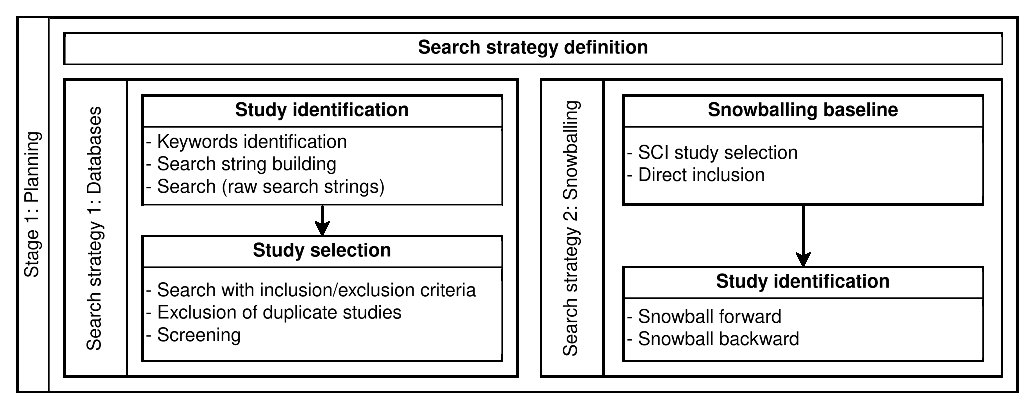
\includegraphics[scale=0.9]{resources/figures/sms-Etapa-1-wide.eps}
	\caption{Activities of the study search stage}
	\label{fig:busqueda-estudios}
\end{figure*}

%sub-subseccion 4.2.1 ------ Defining the Search Strategy
%sub-subseccion 4.2.1 
\subsubsection{Definiendo la Estrategia de Búsqueda}\label{subsubsec:estrategia-busqueda}

Para desarrollar este SMS, se ha implementado una metodología híbrida. Esta metodología tiene como objetivo conseguir una cantidad más amplia de estudios indexados y procedentes de múltiples fuentes, superando los resultados que ofrecen en las bases de datos. De esta manera, integramos dos técnicas de búsqueda. La técnica inicial se denomina ``Búsqueda en bases de datos'' la cual consiste en realizar una búsqueda automatizada dentro de bases de datos académicas indexadas~\cite{Jalai-01}. La técnica secundaria recibe el nombre de \textit{Snowballing} o bola de nieve y representa un procedimiento manual fundamentado en una previa recolección de textos iniciales para identificar investigaciones adicionales mediante sus bibliografías y citaciones~\cite{Jalai-01,Goodman-01}.

Para apoyar el proceso llevado a cabo en este SMS, hemos utilizado los siguientes elementos: a) Bases de datos académicas. b) El software SMS-Builder desarrollado por \cite{Candela2022100935} diseñado específicamente para facilitar la construcción de estudios de mapeo sistemático. c) Herramientas para apoyar la gestión de referencias como Mendeley y la busqueda de las mismas como Google Scholar.

%sub-subseccion 4.2.2 -----  Search Strategy 1: Databases

%%% Variables de frecuencia por cada base de datos. 
\newcommand{\acm}{518}
\newcommand{\ieee}{0}
\newcommand{\sd}{120}
\newcommand{\spr}{209}
\newcommand{\tf}{0}
\newcommand{\tot}{847}
%%% Variables de contrubución porcetual
\newcommand{\acmp}{\fpeval{round(\acm*100/\tot,2)}}
\newcommand{\ieeep}{\fpeval{round(\ieee*100/\tot,2)}}
\newcommand{\sdp}{\fpeval{round(\sd*100/\tot,2)}}
\newcommand{\sprp}{\fpeval{round(\spr*100/\tot,2)}}
\newcommand{\tfp}{\fpeval{round(\tf*100/\tot,2)}}

%%%%% ------------------------------------------------

%%% Variables de frecuencia por cada base de datos. 
\newcommand{\iacm}{315}
\newcommand{\iieee}{0}
\newcommand{\isd}{101}
\newcommand{\ispr}{63}
\newcommand{\itf}{0}
\newcommand{\itot}{479}
%%% Variables de contribución porcentual
\newcommand{\iacmp}{\fpeval{round(\iacm*100/\itot,2)}}
\newcommand{\iieeep}{\fpeval{round(\iieee*100/\itot,2)}}
\newcommand{\isdp}{\fpeval{round(\isd*100/\itot,2)}}
\newcommand{\isprp}{\fpeval{round(\ispr*100/\itot,2)}}
\newcommand{\itfp}{\fpeval{round(\itf*100/\itot,2)}}

%Cantidad de estudios excluídos por ser duplicados
\newcommand{\numEstEx}{3}

%Cantidad de estudios luego de depuración = (estudios totales luego de exclusión - estudios duplicados)
\newcommand{\depTot}{\fpeval{\itot-\numEstEx}}

%Cantidad de estudios depurados por el screening
\newcommand{\screen}{377}
%Cantidad de estudios totales luego del screening
\newcommand{\screenTot}{\fpeval{\depTot-\screen}}

%sub-subseccion 4.2.2
\subsubsection{Search Strategy 1: Databases}

This strategy comprises two components. The first component is termed ``Study Identification''. It focuses on establishing the keywords to construct search strings that enable the completion of queries in digital libraries. The second component is called ``Study Selection''. It focuses on applying various criteria to refine study search results and select those with the most significant value for the SMS\@

\bolditalic{Study Identification}: in order to ensure the feasibility of the SMS and by consensus of the authors, it was decided to limit the number of databases to five, including ACM, IEEE Xplore, Springer, ScienceDirect, Taylor \& Francis. In this part of the process, it is necessary to establish the keywords used subsequently in the search strings for each of the databases. Again, we used the PICOC model as a methodological guide to identify key terms or phrases that serve this purpose. We refined these terms by including synonyms (See Table~\ref{table:picoc_keywords}).

% -------- Tabla : Palabras clave del modelo PICOC. ------------
\begin{table}[htbp]
	\centering
	\caption{Palabras clave identificadas usando el modelo PICOC}
	\label{table:picoc_keywords}
	\renewcommand{\arraystretch}{1}  % Increase row height globally
	\begin{tabular}{p{1.8cm}p{6cm}}
		\toprule
		\textbf{Componente}              & \textbf{Palabras clave}                                                                                                                                                                                                                                                                 \\
		\midrule
		\textbf{Población}               & Universos, HTCondor, Computación distribuida y paralela, HTC, Desarrollo de Software, Virtualización y microservicios, Redes de computadoras, Infraestructura computacional, Inteligencia artificial, Análisis de datos, Pensamiento computacional, Investigación, Docencia, Extensión. \\
		\addlinespace[0.8em]
		\textbf{Intervención}            & Identificación y clasificación.                                                                                                                                                                                                                                                         \\
		\addlinespace[0.8em]
		\textbf{Criterios de aceptación} &
		Casos de proyecto documentados, cumplimiento de criterios de inclusión y exclusión y aparición en bases de datos seleccionadas.                                                                                                                                                                                            \\
		\addlinespace[0.8em]
		\textbf{Salidas}                 & Taxonomía que organiza los trabajos relacionados con la población.                                                                                                                                                                                                                      \\
		\addlinespace[0.8em]
		\textbf{Contexto}                & Universos HTCondor, dominios de computación distribuida y paralela, funciones sustantivas universitarias , investigación, docencia, extensión.                                                                                                                    \\
		\bottomrule
	\end{tabular}
\end{table}
% --------------------------------------------------------------


The selected main keywords were \textit{HTCondor, HTC, Universe, Project, Research}. To broaden the research perspective, we used the Boolean operator ``OR'' to add synonyms to the main keywords.

Finally, the set of keywords selected for the construction of the search string are found in Table~\ref{table:database_search_keywords}.


% -------- Tabla : Palabras clave para búsqueda en base de datos . ------------
\begin{table}[htbp]
	\centering
	\caption{Palabras clave para búsqueda en base de datos}
	\label{table:database_search_keywords}
	\renewcommand{\arraystretch}{1}  % Increase row height globally
	\begin{tabular}{p{1.4cm}p{6.4cm}}
		\toprule
		\textbf{Palabra}  & \textbf{Sinónimos y conceptos relacionados}                \\
		\midrule
		\textbf{HTCondor} & Condor                                                     \\
		\addlinespace[0.8em]
		\textbf{HTC}      & HPC, High Throughput Computing, High Performance Computing \\
		\addlinespace[0.8em]
		\textbf{Universe} & Execution Environment                                      \\
		\addlinespace[0.8em]
		\textbf{Project}  & Work                                                       \\
		\addlinespace[0.8em]
		\textbf{Research} & Teaching, Industry                                         \\
		\bottomrule
	\end{tabular}
\end{table}
% --------------------------------------------------------------





% --------------- Tabla CADENAS DE Búsqueda-----------------------------------------
% -------- Tabla : Cadenas de búsqueda por base de datos ------------
\begin{table*}[htbp]
	\centering
	\caption{Cadenas de búsqueda utilizadas en las bases de datos}
	\label{table:cadenas_de_busqueda}
	\renewcommand{\arraystretch}{1}  % Increase row height globally
	\begin{tabular}{p{3.2cm}p{11cm}p{2.5cm}}
		\toprule
		\textbf{Base de Datos}            & \textbf{Cadena de Búsqueda}                                                                                                                                                                                        & \textbf{Campos}  \\
		\midrule
		\textbf{ACM Full Text Collection} & ((HTCondor OR Condor) AND (HTC OR ``High Throughput Computin'' OR HPC OR ``High Performance Computing'') AND (Universe OR ``Execution Environment'') AND (Project OR Work) AND (Research OR Teaching OR Industry)) & Todos los campos \\
		\addlinespace[0.8em]
		\textbf{IEEE Xplore}              & (HTCondor OR Condor) AND (HTC OR (High Throughput Computing)) AND (Universe OR (Runtime Environment)) AND (Research OR Teaching OR Industry)                                                                       & Todos los campos \\
		\addlinespace[0.8em]
		\textbf{Springer}                 & ((HTCondor | Condor) + (HTC | ``High Throughput Computing'' | HPC | ``High Performance Computing'') + (Universe | ``Execution Environment'') + (Project | Work) + (Research | Teaching | Industry))                & Todos los campos \\
		\addlinespace[0.8em]
		\textbf{ScienceDirect}            & (HTCondor OR Condor) (HTC OR ``High Throughput Computing'' OR HPC OR ``High Performance Computing'') (Universe OR ``Execution Environment'') (Project OR Work) (Research OR Teaching OR Industry)                  & Todos los campos \\
		\addlinespace[0.8em]
		\textbf{Taylor \& Francis}        & (HTCondor OR Condor) AND (HTC OR (High Throughput Computing)) AND (Universe OR (Runtime Environment)) AND (Research OR Teaching OR Industry)                                                                       & Todos los campos \\
		\bottomrule
	\end{tabular}
\end{table*}
% --------------------------------------------------------------


To direct the research toward the intersection of these two groups of terms, the Boolean operator ``AND'' was used. Once we identified the keywords, we continued constructing the search strings for the digital libraries using an iterative process. The iterative construction of search strings consists of performing a heuristic process with keywords, synonyms, and related concepts through the use of disjunctions and conjunctions that conform to the syntactic rules of each database considered in the automated search. Therefore, these strings vary according to the characteristics and functions of each database. See Table~\ref{table:cadenas_de_busqueda}.

After constructing the search strings, these were submitted to each database engine. Table~\ref{table:search_results} shows the set of results obtained. We identified a total of 847 studies preliminarily, with ACM being the largest contributor, delivering the greatest number of results compared to the other databases with \acmp\% of the results.


% -------- Tabla : Resultados de las cadenas de búsqueda ------------


\begin{table*}[htbp]
	\centering
	\caption{Resultados de las cadenas de búsqueda}
	\label{table:search_results}
	\renewcommand{\arraystretch}{1}  % Increase row height globally
	\begin{tabular}{p{4.8cm}p{1.7cm}p{1.7cm}p{1.7cm}p{1.7cm}p{2cm}p{1.4cm}}
		\toprule
		\textbf{Criterios}                                        & \textbf{ACM} & \textbf{IEEE} & \textbf{ScienceDirect} & \textbf{Springer} & \textbf{Taylor\&Francis} & \textbf{Total} \\
		\midrule
		\textbf{Cadena de búsqueda con palabras clave únicamente} & \acm{}       & \ieee{}       & \sd{}                  & \spr{}            & \tf{}                    & \tot{}         \\
		\addlinespace[0.8em]
		\textbf{Contribución porcentual}                          & \acmp{}\%    & \ieeep{}\%    & \sdp{}\%               & \sprp{}\%         & \tfp{}\%                 & 100\%          \\
		\bottomrule
	\end{tabular}
\end{table*}
% --------------------------------------------------------------




\bolditalic{Study Selection}: to refine the results obtained up to this point, we applied the inclusion and exclusion criteria defined in the planning phase. Table~\ref{table:search_results_exclusion} shows the results of this step. After applying said filter, the total number of studies obtained was \itot. According to the different databases consulted, ACM continues to have the most considerable contribution, with \iacmp\% of the studies.

%% Applying duplicate exclusion

From the \itot{} studies selected, the exclusion of three studies was applied given that these were duplicates. After this refinement, the total studies were \depTot{}. From this new dataset, a review named \bolditalic{screening} was conducted, this procedure consists of verifying the title, abstract, and keywords of each study to determine if these are circumscribed within the research context, that is, if they are aligned with the objectives proposed for the SMS. The \textit{screening} process allowed us to discard \screen{} studies given that some of them made reference to different academic disciplines and others were not aligned with the research objectives proposed.

Therefore, we concluded the first search strategy with a total of \screenTot{} studies selected. Figure~\ref{fig:overview} shows an overview of the activities and results obtained in search strategy 1.

\begin{figure}[htbp]
	\centering
	\includegraphics[scale=0.25]{resources/figures/overview.png}
	\caption{Vista general de las actividades y resultados obtenidos en la estrategia de búsqueda por bases de datos}
	\label{fig:overview}
\end{figure}


\begin{table*}[htbp]
	\centering
	\caption{Resultados de las cadenas de búsqueda con criterios de exclusión}
	\label{table:search_results_exclusion}
	\begin{tabular}{p{4.8cm}p{1.7cm}p{1.7cm}p{1.7cm}p{1.7cm}p{2cm}p{1.4cm}}
		\toprule
		\textbf{Criterios}                                        & \textbf{ACM} & \textbf{IEEE} & \textbf{ScienceDirect} & \textbf{Springer} & \textbf{Taylor \& Francis} & \textbf{Total} \\
		\midrule
		\textbf{Cadena de búsqueda con palabras clave únicamente} & \iacm{}      & \iieee{}      & \isd{}                 & \ispr{}           & \itf{}                     & \itot{}        \\
		\addlinespace[0.8em]
		\textbf{Contribución porcentual}                          & \iacmp{}\%   & \iieeep{}\%   & \isdp{}\%              & \isprp{}\%        & \itfp{}\%                  & 100\%          \\
		\bottomrule
	\end{tabular}
\end{table*}
% --------------------------------------------------------------



% sub-subsetion for 4.2.3 --- BUSQUEDA POR SNOWBALL 
% sub-subsetion for 4.2.3 ----- ESTRATEGIA DE BUSQUEDA POR SNOWBALL
\subsubsection{Estrategia de Búsqueda 2: Bola de Nieve (Snowballing)}

\newcommand{\csiSelected}{24} %Estudios identficados con el SCI
\newcommand{\afterCsiTotal}{\fpeval{\screenTot-\csiSelected}} % Estudios totales luegos del SCI


La estrategia de búsqueda de bola de nieve comienza con la identificación del conjunto base de documentos a utilizar, seguido de una revisión y selección de documentos. La revisión consiste en verificar la lista de referencias mediante la identificación de nuevos documentos (bola de nieve hacia atrás). De manera similar, se identifican los documentos que citan el documento revisado (bola de nieve hacia adelante), lo cual requiere el uso de una base de datos que indique esta información. En todos los casos, la sección de documentos aplica los criterios de exclusión \cite{Wohlin-01}.
Esta estrategia comprende dos pasos. El primer paso se denomina ``Construcción de línea base de bola de nieve'' y se enfoca en establecer estudios para iniciar el análisis de referencias y citas. Para la composición de este conjunto de estudios, utilizamos varios criterios basados en el CVI (Índice de Valor de Contenido), SCI (Índice de Citas de Estudios), además de también usar la inclusión directa. El segundo paso se denomina ``Selección de estudios'', y se enfoca en el análisis de referencias (Bola de nieve hacia atrás) y citas (Bola de nieve hacia adelante) de cada estudio.


% Snowball baseline building 
\bolditalic{Construcción de línea base de bola de nieve}: Basándose en los \screenTot{} estudios seleccionados, realizamos un análisis de frecuencia con el cuál obtuvimos \csiSelected{} estudios por medio del índice SCI con, dando un total de \afterCsiTotal{} estudios. 
% ---- No hicimos ninguna inclusión directa. 
%Como parte del proceso seguido para realizar el SMS, es posible incluir estudios directamente. Esta inclusión directa permite flexibilidad en el método seguido al considerar estudios fuera de los criterios de exclusión. En nuestro caso particular, se incluyeron tres estudios del tipo proceedings.


% Creo que no tomamos en cuenta el CVI y dado que tampoco hicimos inclusión directa, el siguiente parrafo sobra. 
% El total de los estudios identificados por CVI (XXXX), SCI (XXXXXXXX), e inclusión directa (XXXXXXXX) suman XXXXXXXX y constituyen la línea base para el inicio de la bola de nieve.


\bolditalic{Selección de estudios}: Comenzamos con una iteración hacia atrás revisando en cada uno de los XXXX estudios las referencias existentes. Esta revisión nos permitió identificar nuevos artículos que cumplen con los requisitos de inclusión. El resultado fue XXXXXXXX nuevos estudios.
Posteriormente hicimos una iteración hacia adelante revisando aquellos estudios que citan los documentos de línea base. Esta actividad se realizó a través de Google Scholar y siguiendo la práctica en el estudio [XXXX]. El resultado de esta actividad fue XXXXXXXX nuevos estudios. En total, la estrategia de búsqueda de bola de nieve permitió la identificación de XXXXXXXX estudios, XXXXXXXX de ellos a través de iteraciones Hacia adelante-Hacia atrás y tres estudios que integramos por inclusión directa. Ver Fig. XXXXXXXX.


% sub-subsetion for 4.2.4 -- RESULTADOS DE LA BUSQUEDA DE ESTUDIOS
\newcommand{\totalEtapaDos}{\fpeval{\screenTot + \snowballNewStudies}}
\newcommand{\dbPercentEtapa}{\fpeval{round(\screenTot*100/\totalEtapaDos,2)}}
\newcommand{\snowPercentEtapa}{\fpeval{round(\snowballNewStudies*100/\totalEtapaDos,2)}}

% sub-subsection 4.2.4
\subsubsection{Study Search Results}\label{subsubsec:resultados-busqueda}

Finally, adding the \snowballNewStudies{} studies obtained in the snowball process to the \screenTot{} previously obtained with the database search strategy, a total of \totalEtapaDos{} studies is obtained for this stage. See Table~\ref{table:resultados_etapa_2}.

% -------- Table : Results of stage 2: Study search ------------
\begin{table}[htbp]
	\centering
	\caption{Results of stage 2: Search for studies}
	\label{table:resultados_etapa_2}
	\renewcommand{\arraystretch}{1}  % Increase row height globally
	\begin{tabular}{p{2.5cm}p{2.6cm}p{2.5cm}}
		\toprule
		\textbf{Strategy} & \textbf{Studies}      & \textbf{\%}           \\
		\midrule
		Databases         & \screenTot{}          & \dbPercentEtapa{}\%   \\
		\addlinespace[0.8em]
		Snowballing       & \snowballNewStudies{} & \snowPercentEtapa{}\% \\
		\addlinespace[0.8em]
		Total             & \totalEtapaDos        & 100\%                 \\
		\bottomrule
	\end{tabular}
\end{table}
% --------------------------------------------------------------
